\begin{frame}
    \frametitle{Modos de juego}

    \begin{columns}

        \column{170px}

        \begin{block}{Carrera rápida}
            \begin{itemize}
                \item Jugador contra tres oponentes
                \item Número de vueltas deseadas
                \item Una única carrera
            \end{itemize}
        \end{block}

        \begin{block}{Campeonato}
            \begin{itemize}
                \item Jugador contra tres oponentes
                \item Cuatro circuitos a completar
                \item Número de vueltas deseadas
                \item Puntuación
            \end{itemize}
        \end{block}

        \begin{block}{Contrarreloj}
            \begin{itemize}
                \item Jugador compite solo
                \item Sólo ítems de turbo
                \item Tres vueltas al circuito
            \end{itemize}
        \end{block}

        \column{130px}
        
        \begin{center}
                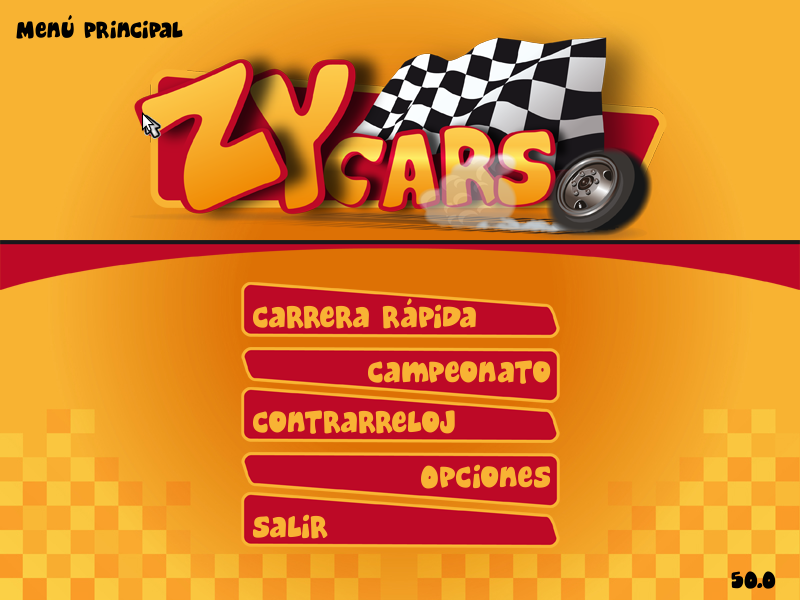
\includegraphics[scale=0.17]{imagenes/menuprincipal.png}
        \end{center}

    \end{columns}
    
\end{frame}

\begin{frame}
    \frametitle{Elementos del juego}

    \begin{columns}

        \column{180px}
        
        \begin{block}{Personajes}
            \begin{itemize}
                \item Variedad
                \item Distintas características (tamaño, velocidad...)
                \item Ampliables
            \end{itemize}
        \end{block}
        
        \begin{block}{Bolas de ítems}
            \begin{itemize}
                \item A lo largo de todos los circuitos
                \item Proporcionan un ítem aleatorio
            \end{itemize}
        \end{block}
        
        \begin{block}{Tipos de ítems}
            \begin{itemize}
                \item Ataques a distancia
                \item Obstáculos
                \item Velocidad
            \end{itemize}
        \end{block}

        \column{120px}

        \begin{center}
                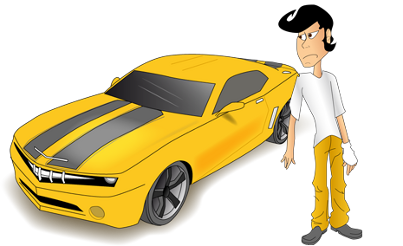
\includegraphics[scale=0.3]{imagenes/ejemplo_personaje.png}
        \end{center}

        \begin{center}
                
\includegraphics[scale=0.5]{imagenes/item_box.png}
        \end{center}
        
    \end{columns}

\end{frame}

\begin{frame}
    \frametitle{Colaboración y Recursos}

        \begin{block}{Diseño Gráfico}
        Se ha contado con la colaboración de David Nieto Rojas, quien ha colaborado en el apartado gráfico del juego.
        \end{block}
        
        \begin{columns}
        
            \column{150px}
            \begin{block}{Música}
            Se usa música libre adecuada para el videojuego. Grupos:
                \begin{itemize}
                    \item Bob Wizman
                    \item Pirato Ketchup
                    \item Los Cadaver
                    \item The Wavers
                    \item Zamalska 
                \end{itemize}
            \end{block}
            
            \column{150px}
            \begin{center}
                    
\includegraphics[scale=0.05]{imagenes/logo_jamendo.png}
            \end{center}
            
        \end{columns}

\end{frame}

